\documentclass{beamer}
\usetheme{Warsaw}

\usepackage[utf8]{inputenc}
\usepackage{fancybox}
\usepackage{multimedia} 
\usepackage{subfig}
\usepackage{amsmath}
\usepackage{hyperref}
\usepackage[all]{xy}
\usepackage{algorithm}
%\usepackage{arevmath}     % For math symbols
\usepackage[noend]{algpseudocode}

\begin{document}


\title[Angewandte Mathematik] % (optional, only for long titles)
{Angewandte Mathematik
\\
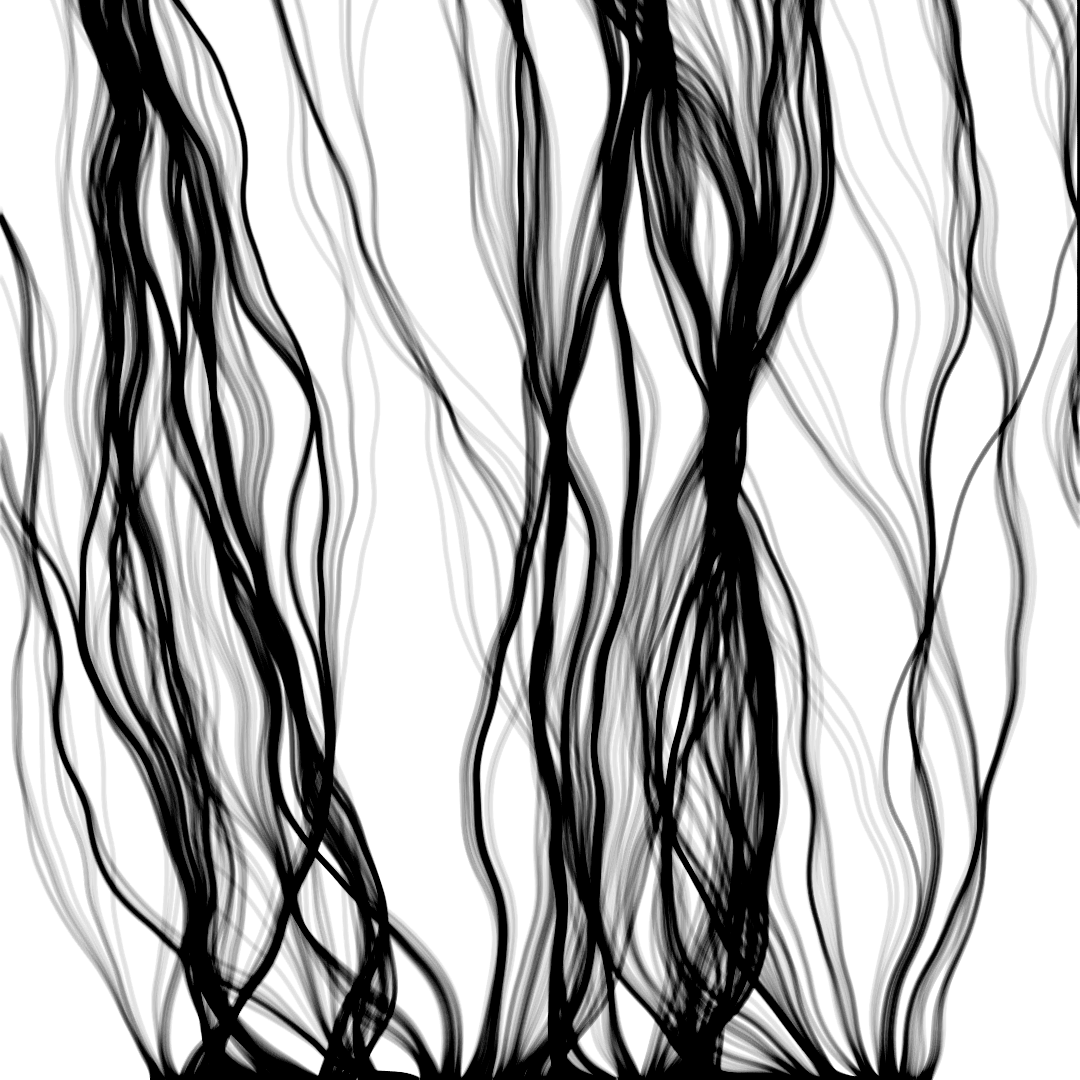
\includegraphics[scale=0.15]{images/cover}
}
\subtitle{}
\author[Dr. Johannes Riesterer] % (optional, for multiple authors)
{Dr.  rer. nat. Johannes Riesterer}

\date[KPT 2004] % (optional)
{}

\subject{Angewandte Mathematik}



\frame{\titlepage}

\begin{frame}
    \frametitle{Digitale Bilder}
\framesubtitle{}
    \begin{block}{Umwandlung von Bildern}
\begin{itemize}
\item Viele Verfahren der  Signalverarbeitung haben ihren Ursprung in der Analysis. Um diese anwenden zu können, müssen diskrete Daten  in kontinuierliche Daten umgewandelt werden.
\item Auf der anderen Seite kann  ein Computer nur diskrete Daten  verarbeitet. Kontinuierliche Signale (zum Beispiel von Sensoren) müssen daher in diskrete Daten umgewandelt werden.
\end{itemize}
\end{block}

 \end{frame}

\begin{frame}
    \frametitle{Digitale Bilder}
\framesubtitle{}
    \begin{block}{}
Für ein eindimensionales, diskretes Bild $U : [1, \ldots, N]  \to R$ bezeichne  $U_{j} := U(j)$.
\end{block}
    \begin{block}{Stückweise konstante Interpolation}
Definiere $\phi^0 (x) : = 1_{ [-\frac{1} {2} ,  \frac{1} {2}) }(x) : =\begin{cases}
   1 , & \text{for } -\frac{1} {2}  \leq x < \frac{1} {2}  \\
    0  & \text{else } 
  \end{cases} $, $\phi^0_j(x):= \phi^0 (x - j)$ und
 $u(x) := \sum_{j=1}^{N} U_j \phi^0_j(x)$ 
\end{block}

 \end{frame}





\begin{frame}
    \frametitle{Digitale Bilder}
\framesubtitle{}
\begin{block}{Höherdimensionale stückweise  Interpolation}
Für ein 2-dimensionales, diskretes Bild $U : [1, \ldots, N] \times   [1, \ldots, M] \to R$ definiere 
 $u(x, y) := \sum_{i=1}^{N} \sum_{j=1}^{M}  U_{i,j} \cdot \phi_i(x) \cdot \phi_j(y)$ und analog für n-dimensonale Bilder....
\end{block}
 \end{frame}


\begin{frame}
    \frametitle{Digitale Bilder}
\framesubtitle{}
\begin{block}{Abtastung}
Für ein kontinuierliches  Bild $u : I^n \to R$ erhält man durch gewichtete Mittelungen
$U_i := \int_{I^n} \phi (x - x_i) u(x) dx$ ein diskretes Bild. 
\end{block}
 \end{frame}


\begin{frame}
    \frametitle{Integration}
\framesubtitle{}

    \begin{block}{Faltung}
\begin{align}
(f * g )(x) := \int_{\mathbb{R}^n}  f(y-x) \cdot g(y) \; dy 
\end{align}

\end{block}
    \begin{block}{Beispiel 1}
\href{https://moodle.dhbw-mannheim.de/pluginfile.php/278535/mod_folder/content/0/Convolution_of_box_signal_with_itself.gif?forcedownload=1}{Link: Box}
\end{block}
 
    \begin{block}{Beispiel 2}
\href{https://moodle.dhbw-mannheim.de/pluginfile.php/278535/mod_folder/content/0/Convolution_Animation_(Gaussian).gif?forcedownload=1}{Link: Gauß}
\end{block}
 
\end{frame}


\begin{frame}
    \frametitle{Diskrete Faltung}
\framesubtitle{}

    \begin{block}{Diskrete Faltung}
Für zwei diskrete  Funktionen $U : [1, \ldots, N]  \to R$ und $H : [1, \ldots, N]  \to R$ mit stückweisen konstanten Interpolation $u(x) := \sum_{l=1}^{N} U_l \phi^0_j(x)$ und 
$h(x) := \sum_{m=1}^{N} H_m \phi^0_m(x)$ ergibt die Faltung 
\begin{align*}
& (h * u)(k) = \int u(y)h(k-y)  \; dy \\
& = \int \ \sum_{l=1}^{N} U_l \phi^0(y-l) \sum_{m=1}^{N} H_m \phi^0(k-y-m) \\
& = \sum_{l=1}^{N}   \sum_{m=1}^{N} U_l  H_m  \int  \phi^0(y-l) \phi^0(k-y-m) \; dy 
\end{align*}

\end{block}
 \end{frame}

\begin{frame}
    \frametitle{Diskrete Faltung}
\framesubtitle{}

    \begin{block}{Diskrete Faltung}
Da für das Integral 
\begin{align*}
  \int  \phi^0(y-l) \phi^0(k-y-m)  \; dy  = \begin{cases}
1 \text{ falls } m = k -l\\
0 \text{ sonst }
\end{cases}
\end{align*}
gilt, folgt die Darstellung
\begin{align*}
 (u  * h)(k) = \sum_l U_l H_{k-l}
\end{align*}

\end{block}

 \end{frame}


\begin{frame}
    \frametitle{Kantenerkennung}
\framesubtitle{}
\begin{block}{Kanten}
Kanten sind durch schnelle Änderungen des Farbwertes gekennzeichnet. Sie sind damit Extremstellen der ersten Ableitung.
\end{block}
\begin{figure}[htp]
      \centering
Intensität und Gradient entlang eines Bildschnittes \\
    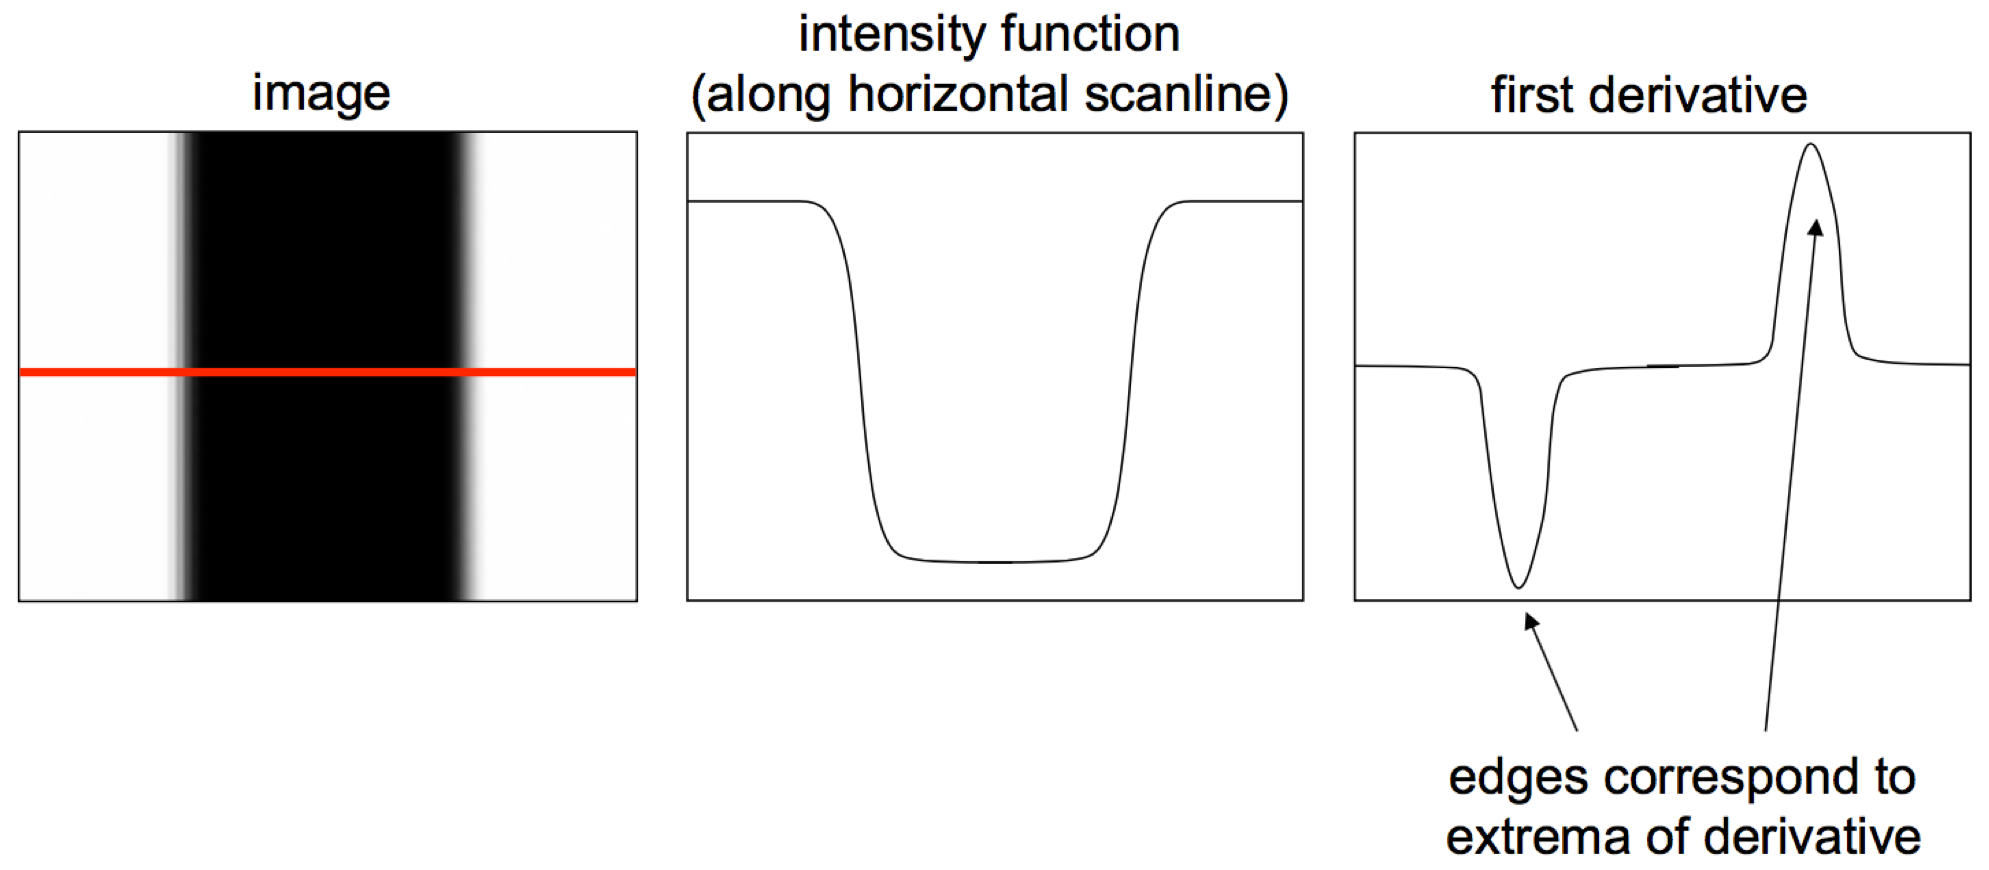
\includegraphics[width=0.65\textwidth]{images/edgedetection} 
      \caption{Quelle: ai.stanford.edu}
\end{figure}

 \end{frame}

\begin{frame}
    \frametitle{Kantenerkennung}
\framesubtitle{}
\begin{block}{Gradientenbasierte Kantenerkennung}
Bei der Detektion von Kanten mit Hilfe des Gradienten ist   Rauschen ein Problem, da sich  hier ebenfalls  der Farbwert schnell ändert. 
\end{block}
\begin{figure}[htp]
      \centering
Rauschen \\
    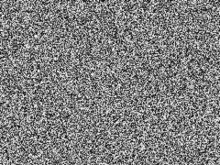
\includegraphics[width=0.45\textwidth]{images/noise} 
      \caption{Quelle: Wikipedia}
\end{figure}

 \end{frame}

\begin{frame}
    \frametitle{Kantenerkennung}
\framesubtitle{}
\begin{block}{Gradientenbasierte Kantenerkennung}
Idee: Wende einen Filter an, der das Rauschen reduziert und bilde dann den Gradienten. Bilde also den Gradienten
\begin{align*}
\frac{\partial (u * f)(x)}{\partial x} 
\end{align*}
wobei $f$ ein Faltungskern ist.
\end{block}

\begin{block}{Ableitung von Faltungen}
Es gilt
\begin{align*}
\frac{\partial (u * f)(x)}{\partial x} = (u * f')(x)
\end{align*}

\end{block}

 \end{frame}


\begin{frame}
    \frametitle{Kantenerkennung}
\framesubtitle{}
\begin{block}{Gradientenbasierte Kantenerkennung}
Welcher Filter ist gut geeignet?
\end{block}
\begin{block}{Kantenerkennung nach Canny}
Es gibt Kanten auf unterschiedlichen Skalen ("grobe Kanten" und "feine Kanten"). Wähle daher einen parameterabhängigen Faltungskern
$f_\sigma$. Zu einem Originalbild $u_0$ bekommen wir eine ganze Klasse von Bildern
\begin{align*}
u(x, \sigma) = u_0 * f_\sigma(x) \;.
\end{align*}
 \end{block}

 \end{frame}

\begin{frame}
    \frametitle{Kantenerkennung}
\framesubtitle{}

\begin{block}{Kantenerkennung nach Canny}
Die Stellen der Kanten soll sich bei wachsendem $\sigma$ nicht verändern und ebenso sollen auch keine Kanten hinzukommen. 
Deswegen soll in einem Kantenpunkt $x_0$ von $u_0$ gelten:
\begin{align*}
\frac{\partial^2}{\partial x^2} > 0 \Rightarrow \frac{\partial}{\partial \sigma}  u(x_0, \sigma) > 0 \\
\frac{\partial^2}{\partial x^2} = 0 \Rightarrow \frac{\partial}{\partial \sigma}  u(x_0, \sigma) = 0 \\
\frac{\partial^2}{\partial x^2} < 0 \Rightarrow \frac{\partial}{\partial \sigma}  u(x_0, \sigma) <0
\end{align*}
 \end{block}

 \end{frame}

\begin{frame}
    \frametitle{Kantenerkennung}
\framesubtitle{}

\begin{block}{Kantenerkennung nach Canny}
Für einen allgemeinen Punkt soll daher gelten:
\begin{align*}
&\frac{\partial^2}{\partial x^2}  u(x, \sigma)  =  \ \frac{\partial}{\partial \sigma}  u(x, \sigma)  \\
&  u(x, 0) = u_0(x) 
\end{align*}
 \end{block}

\begin{block}{Kantenerkennung nach Canny}
Diese partielle Differentialgleichung hat die eindeutige Lösung
\begin{align*}
&  u(x, \sigma) = (u_0 * G^{\sqrt{2\sigma}}) (x)
\end{align*}
wobei $ G^{\sqrt{2\sigma}}$ der Gaußfilter ist.
 \end{block}

 \end{frame}


\begin{frame}
    \frametitle{Kantenerkennung}
\framesubtitle{}

\begin{block}{Kantenerkennung nach Canny}
Die Kantenerkennung nach Canny faltet ein gegebenes Bild $u$ zuerst mit einem Gaußkernel $G^{\sigma}$. Danach wird  der Betrag der Ableitung und seine Richtung berechnet: 
\begin{align*}
p(x) = & || \nabla (u * G^\sigma)(x) || \\
&= \sqrt{ (\frac{\partial}{\partial x_1} (u * G^\sigma)(x))^2 + (\frac{\partial}{\partial x_2} (u * G^\sigma)(x))^2 } \\
\theta(x) & = \angle  \nabla (u * G^\sigma)(x) = \arctan \biggl( \frac{\frac{\partial}{\partial x_2} (u * G^\sigma)(x)}{\frac{\partial}{\partial x_1} (u * G^\sigma)(x)} \biggr)
\end{align*}


 \end{block}

 \end{frame}



\begin{frame}
    \frametitle{Kantenerkennung}
\framesubtitle{}
\begin{block}{Kantenerkennung nach Canny}
Als Kanten werden lokale Maxima von $p(x)$ in Richtung $(\sin \theta(x), \cos \theta(x)  )$
\end{block}
\begin{figure}[htp]
      \centering
Kanten als lokale Maxima in Kantenrichtung \\
    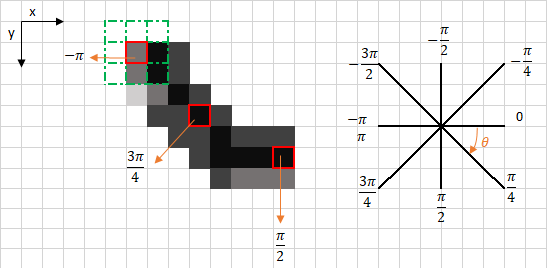
\includegraphics[width=0.55\textwidth]{images/canny_max} 
      \caption{Quelle: towardsdatascience.com}
\end{figure}

 \end{frame}




\begin{frame}
    \frametitle{Kantenerkennung}
\framesubtitle{}
\begin{block}{Kantenschärfen mit Laplace}
Durch die Operation $u - \tau \bigtriangleup u$ werden die Kanten hervorgehoben.
\end{block}
\begin{figure}[htp]
      \centering
Kanten als lokale Maxima in Kantenrichtung \\
    \includegraphics[width=0.55\textwidth]{images/laplace1} \\
    \includegraphics[width=0.35\textwidth]{images/laplace2} 
      \caption{Quelle:OpenCV}
\end{figure}
 \end{frame}

\begin{frame}
    \frametitle{Kantenerkennung}
\framesubtitle{}
\begin{figure}[htp]
      \centering
Kantenschärfung \\
    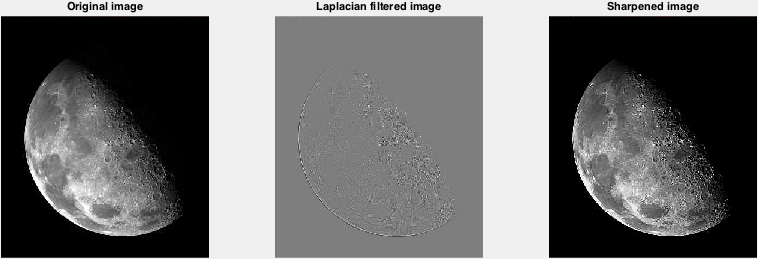
\includegraphics[width=0.95\textwidth]{images/sharpening} 
      \caption{Quelle: Stackoverflow}
\end{figure}
 \end{frame}



\end{document}

